%% LyX 2.4.2.1 created this file.  For more info, see https://www.lyx.org/.
%% Do not edit unless you really know what you are doing.
\documentclass[english,compress]{beamer}
\usepackage[latin9]{inputenc}
\setcounter{secnumdepth}{3}
\setcounter{tocdepth}{3}
\usepackage[active]{srcltx}
\usepackage{booktabs}
\usepackage{amsbsy}
\usepackage{amstext}
\usepackage{graphicx}
\usepackage{comment}
\usepackage[authoryear]{natbib}
\PassOptionsToPackage{normalem}{ulem}
\usepackage{ulem}

\setbeamertemplate{blocks}[rounded][shadow=false]

\makeatletter

%%%%%%%%%%%%%%%%%%%%%%%%%%%%%%% LyX specific LaTeX commands.
%% Because html converters don't know tabularnewline
\providecommand{\tabularnewline}{\\}

%%%%%%%%%%%%%%%%%%%%%%%%%%%%%%% Textclass specific LaTeX commands.
% this default might be overridden by plain title style
\newcommand\makebeamertitle{\frame{\maketitle}}%
% (ERT) argument for the TOC
\AtBeginDocument{% 
  \let\origtableofcontents=\tableofcontents
  \def\tableofcontents{\@ifnextchar[{\origtableofcontents}{\gobbletableofcontents}}
  \def\gobbletableofcontents#1{\origtableofcontents}
}

%%%%%%%%%%%%%%%%%%%%%%%%%%%%%%% User specified LaTeX commands.
\usepackage{eurosym}
\usepackage[english]{babel}
\usepackage{metalogo}
\usepackage{listings}
\usepackage{fontspec}
\usepackage{tikz}
\usepackage{colortbl}
\usetikzlibrary{patterns}
\usetikzlibrary{decorations}

\usetheme{Nord}

\AtBeginSection[]
{
  \begin{frame}[c,noframenumbering,plain]
    \tableofcontents[sectionstyle=show/hide,subsectionstyle=show/show/hide]
  \end{frame}
}

\AtBeginSubsection[]
{
  \begin{frame}[c,noframenumbering,plain]
    \tableofcontents[sectionstyle=show/hide,subsectionstyle=show/shaded/hide]
  \end{frame}
}

% Kill to take pages out
\setbeamertemplate{footline}{
  \hfill%
  \usebeamercolor[fg]{page number in head/foot}%
  \scriptsize\insertframenumber{} / \inserttotalframenumber%
  \hspace{1em}\vspace{1em}
}

\title[Portfolio Theory with Settlement Frictions]{Portfolio Theory w/ Settlement Frictions}
\author{Javier Bianchi (FRB-Min) \and Saki Bigio (UCLA \& NBER)}


\date{UCLA Workshop -- July 2025}

\begin{document}

\makebeamertitle

\begin{frame}{Big Picture \& Agenda}
\begin{itemize}
    \item \textbf{Recent macro-finance:} convenience yields
    \begin{itemize}
        \item Treasuries, Repo, FX markets
    \end{itemize}
    \medskip
    \item \textbf{Convenience yields:} premia unexplained by cash flow (risk)
    \medskip
    \item \textbf{Agenda:} links convenience yields to
    \begin{itemize}
        \item Supply of settlement instruments (e.g., reserves, debt)
        \item OTC market frictions
    \end{itemize}
    \medskip
    \item \textbf{Why Microfoundations?}
    \begin{enumerate}
        \item Testable micro predictions: volumes, rates, dispersion
        \item Policy-relevance: non-invariant to policy
        \item Interaction with risk-aversion
    \end{enumerate}
\end{itemize}
\end{frame}

\begin{frame}{Preview of Mechanism}
\begin{itemize}
    \item Investors with portfolios
    \item Cash-flows:
    \textbf{settlement shocks} (e.g., deposits, margin calls)
    \item \textbf{Cash deficit:} borrow in \textbf{OTC market} or face penalty rate
    \item \textbf{Kinked convenience-yield function} of cash position s: 
    \[
    \chi(s) = \begin{cases}
        \chi^- s & \text{if } s < 0 \\
        \chi^+ s & \text{if } s \geq 0
    \end{cases}
    \]
    \item \(\chi^-\) and \(\chi^+\) depend on:
    \begin{itemize}
        \item market tightness \(\theta = S^-/S^+\)
        \item matching technology \(G,\bar{\lambda}\)
        \item bargaining power \(\eta\)
    \end{itemize}
\end{itemize}
\end{frame}

\begin{frame}{Preview of Mechanism}
\begin{figure}[h]
\centering
\begin{minipage}{0.4\textwidth}
\centering
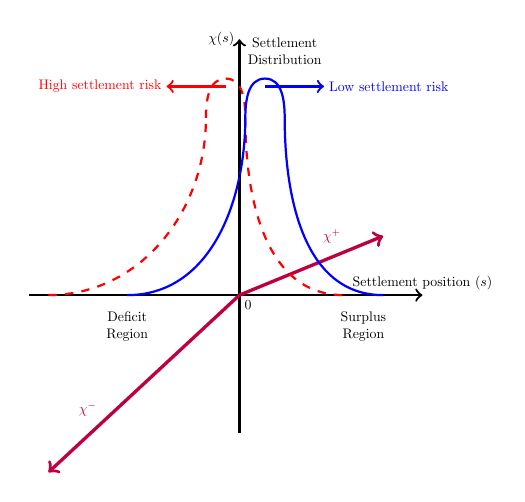
\begin{tikzpicture}[thick,scale=0.5, every node/.style={transform shape}]
% First figure (original)
% Axes
\draw[->, black] (-2,0) -- ( 8, 0) node[above]{Settlement position $(s)$};
\draw[->, black] (3.35,-3.5) -- (3.35, 6.5) node[left]{$\chi(s)$};
% Zero point
\node[black, below right] at (3.35,0){$0$};
% Region labels (below x-axis)
\node[align=center,black] at (6.5,-0.8){Surplus\\Region};
\node[align=center,black] at (0.5,-0.8){Deficit\\Region};
\node[align=center,black] at (4.5,6.2){Settlement\\Distribution};
% Liquidity yield function (concave, kinked at origin)
\draw[<-, very thick, purple] (-1.5,-4.5) -- (3.35, 0); % Steep negative slope for deficit
\draw[->, very thick, purple] (3.35,0) -- (7,1.5); % Gentle positive slope for surplus
% Distribution curves (no shading)
\draw[red, dashed] (-1.5,0) to [out=0,in=-90] (2.5,4.5);
\draw[red, dashed] (2.5,4.5) to [out=90,in=180] (3.0,5.5);
\draw[red, dashed] (3.0,5.5) to [out=0,in=90] (3.5,4.5);
\draw[red, dashed] (3.5,4.5) to [out=-90,in=180] (6.0,0);
\draw[blue,thick] (0.5,0) to [out=0,in=-90] (3.5,4.5);
\draw[blue, thick] (3.5,4.5) to [out=90,in=180] (4.0,5.5);
\draw[blue, thick] (4.0,5.5) to [out=0,in=90] (4.5,4.5);
\draw[blue, thick] (4.5,4.5) to [out=-90,in=180] (7.0,0);
% Labels for distributions (moved away from y-axis)
\draw[red,thick,->] (3.0,5.3) -- (1.5,5.3) node[left]{High settlement risk};
\draw[blue,thick,->] (4.0,5.3) -- (5.5,5.3) node[right]{Low settlement risk};
% Slopes labels
\node[purple] at (-0.5,-2.9) {$\chi^-$};
\node[purple] at (5.7,1.5) {$\chi^+$}; % Moved closer to the curve
% Vertical line at zero
\draw[black, dotted] (3.35,-3.5) -- (3.35,6.5);
\end{tikzpicture}
\center{(a) Convenience yields}
\end{minipage}
\hspace{1cm}
\begin{minipage}{0.4\textwidth}
\centering
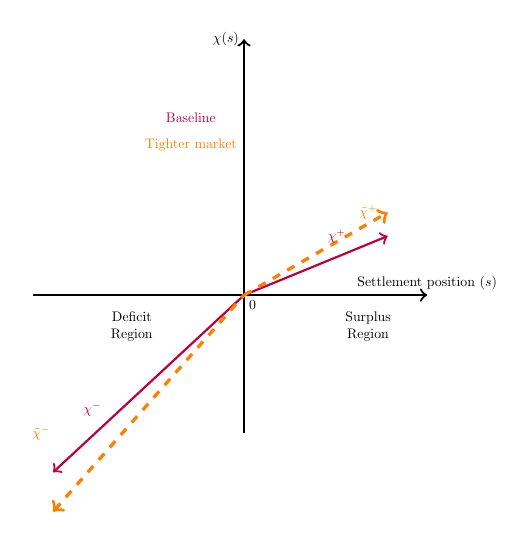
\begin{tikzpicture}[thick,scale=0.5, every node/.style={transform shape}]
% Second figure (with rotation)
% Axes
\draw[->, black] (-2,0) -- ( 8, 0) node[above]{Settlement position $(s)$};
\draw[->, black] (3.35,-3.5) -- (3.35, 6.5) node[left]{$\chi(s)$};
% Zero point
\node[black, below right] at (3.35,0){$0$};
% Region labels (below x-axis)
\node[align=center,black] at (6.5,-0.8){Surplus\\Region};
\node[align=center,black] at (0.5,-0.8){Deficit\\Region};
% Original liquidity yield function
\draw[<-, thick, purple] (-1.5,-4.5) -- (3.35, 0);
\draw[->, thick, purple] (3.35,0) -- (7,1.5);
% Rotated liquidity yield function (tighter market)
\draw[<-, very thick, orange, dashed] (-1.5,-5.5) -- (3.35, 0);
\draw[->, very thick, orange, dashed] (3.35,0) -- (7,2.1);
% Slopes labels for original function
\node[purple] at (-0.5,-2.9) {$\chi^-$};
\node[purple] at (5.7,1.5) {$\chi^+$};
% Slopes labels for rotated function
\node[orange] at (-1.8,-3.5) {$\tilde{\chi}^-$};
\node[orange] at (6.5,2.1) {$\tilde{\chi}^+$};
% Legend
\node[purple] at (2,4.5) {Baseline};
\node[orange] at (2,3.8) {Tighter market};
% Vertical line at zero
\draw[black, dotted] (3.35,-3.5) -- (3.35,6.5);
\end{tikzpicture}
\center{(b) Tightness and convenience yields}
\end{minipage}
% \caption{Liquidity yield function $\chi(s)$ and portfolio choice. Panel (a) shows how different portfolio volatilities interact with the kinked liquidity yield function. Panel (b) illustrates how market tightness (driven by others' portfolio choices) rotates the liquidity yield function, increasing both borrowing costs and lending returns.}
%\label{fig:liquidity_yields}
\end{figure}
\end{frame}

\begin{frame}{What we do here}
    \begin{itemize}
        \item Afonso-Lagos ECMA '15 
        \begin{itemize}
        \item OTC market for Fed Funds
        \end{itemize}
        \medskip
        \item  Bianchi-Bigio ECMA '22
        \begin{itemize}
        \item analytic OTC model (Leontief matching) \item embedded in GE 
        \item study monetary policy
        \end{itemize}
        \medskip
        \item Novelty here:
        \begin{itemize}        
            \item arbitrary assets (not only deposits)
            \item generalize matching function 
            \item comparative statics convenience-yields
        \end{itemize}
    \medskip
    \item Input in Recent work: 
        \begin{itemize}
            \item applications to exchange rates
            \item optimal size of central-bank balance sheets
        \end{itemize}
    \end{itemize}
\end{frame}

\begin{frame}{Contributions here}
\begin{enumerate}
    \item \textbf{Portfolio Theory:}
    \begin{itemize}
    \item integrate OTC friction into rich asset choice/asset pricing framework
    \end{itemize}
    \medskip
    \item \textbf{OTC Market:} 
    \begin{itemize}
    \item formulas for trading rates \& volumes for various cases 
    \item focus identification w/ micro data
    \end{itemize} 
    \medskip
    \item \textbf{Asset Pricing:} theory of convenience yields 
    \begin{itemize}
    \item details how convenience yields vary with market structure/quantities
    \end{itemize} 
    \medskip
    \item \textbf{Normative:} Identifies inefficient portfolio choices: guide regulation
\end{enumerate}
\end{frame}

\section{Environment}

\begin{frame}{Model Environment}
\begin{itemize}
  \item Infinite-horizon, unit mass of investors
  \item Asset return risk and \textbf{settlement risk}
  \item Trade in settlement instrument \textbf{frictional OTC market}
  \item Failure to borrow: penalty rate
\end{itemize}
\end{frame}

\begin{frame}{Timeline: Two-Stages}
\begin{enumerate}
  \item \textbf{Portfolio Stage}
  \begin{itemize}
    \item Choose holdings in assets $\{a^i\}$, $i\in\mathcal{I}$, and cash $m$
  \end{itemize}
  \medskip
  \item \textbf{Balancing Stage}
  \begin{itemize}
    \item Idiosyncratic cash-flow shocks $\omega^i$
    \item Settlement in cash $m$
    \item OTC trade: Borrow (or lend) from other investors $f$ and or amount $w$ at penalty (lender of last resort)
  \end{itemize}
\end{enumerate}
\end{frame}

\begin{frame}{Asset Structure}
\begin{itemize}
  \item Assets $\{a^i\}_{i \in \mathbb{I}}$ differ in payoffs and liquidity properties
  \item Special asset $m$: riskless  
  \item Constraint: must end each period $m \geq 0$
\end{itemize}
\end{frame}

\begin{frame}{Cash-Flow Shocks and Surplus Definition}
\begin{itemize}
  \item At balancing stage, shocks $\omega^i$ perturb asset positions:
  \[
  a_{t+1}^i = \tilde{a}_{t+1}^i (1 + \omega_t^i)
  \]
  \item Settlement surplus:
  \[
  s = \tilde{m}_{t+1} + \sum_i \frac{R_{t+1}^i}{R_{t+1}^m} \omega_t^i \tilde{a}_{t+1}^i
  \]
  \item $s < 0$: deficit \(\rightarrow\) needs funding
  \item $s > 0$: surplus \(\rightarrow\) can lend or hold
  \item Examples: deposits, credit lines, margin calls, insurance claims, refinancing options, etc.
\end{itemize}
\end{frame}

\begin{frame}{OTC trade}
\begin{itemize}
  \item Deficits funded via:
  \begin{itemize}
    \item OTC market borrowing (probability $\Psi^-_t$)
    \item At penalty (probability $1 - \Psi^-_t$)
  \end{itemize}
  \medskip
  \item Surplus lent in OTC market (probability $\Psi^+_t$)
  \medskip
  \item Final cash holdings:
  \[
  m_{t+1} = s + f_{t+1} + w_{t+1} \ge 0
  \]
\end{itemize}
\end{frame}

\begin{frame}{Convenience Yields from Settlement Risk}
\begin{itemize}
  \item Total return includes direct asset return + settlement yield:
  \[
  e_{t+1} = \sum_i R_{t+1}^i \tilde{a}_{t+1}^i + R_{t+1}^m \tilde{m}_{t+1} + \chi_{t+1}(s)
  \]
  \medskip
  \item Kinked convenience-yield function:
  \[
  \chi_t(s) = \begin{cases}
    \chi_t^- s & \text{if } s < 0 \\
    \chi_t^+ s & \text{if } s \ge 0
  \end{cases}
  \]
  \item Slopes depend on equilibrium OTC outcomes:
  
  \[\chi_t^- = (\bar{R}_t^f - R_t^m) \Psi_t^- + (R_t^w - R_t^m)(1 - \Psi_t^-) 
  \]

  \[
  \chi_t^+ = (\bar{R}_t^f - R_t^m) \Psi_t^+
  \]
  \medskip
  \item $\bar{R}_t^f$: average OTC rate, $R_t^w$: penalty rate
  \item Notation: $r^x$ lower case for net rate
\end{itemize}
\end{frame}

\section{OTC Market and Its Equilibrium}
\subsection{Sequential Trade}
\begin{frame}{OTC Market Equilibrium: Matching Dynamics}
\begin{itemize}
  \item Afonso-Lagos block 
  \item Define initial \textbf{aggregate} surplus and deficit:
  \[
  S_0^+ = S^+, \quad S_0^- = S^-
  \]
  \item $n\in\mathcal{N}\equiv\{1,2,...,N\}$ rounds
  \item Round $n$, number of matches:
  \[
  m_n = \lambda_N G(S_n^+, S_n^-)
  \]
  \item Surplus and deficit evolve as:
  \[
  S_{n+1}^+ = S_n^+ - m_n, \quad S_{n+1}^- = S_n^- - m_n
  \]
\end{itemize}
\end{frame}

\begin{frame}{Assumptions on  Matching Function}
Assume: 
\begin{itemize}
  \item \textbf{No disposal:} \( G(0,1) = G(1,0) = 0 \)
  \item \textbf{Constant returns to scale:} Homogeneous degree one
  \item \textbf{Symmetry:} \( G(a,b) = G(b,a) \)
  \item \textbf{Weak exhaustion:} \( \lambda_N G(S_n^+, S_n^-) \leq \min\{S_n^+, S_n^-\} \)
  \item \textbf{Monotonicity:} \( G_a, G_b \geq 0 \)
  \item \textbf{Weak concavity:} \( G_{aa}, G_{bb} \leq 0 \)
\end{itemize}
\medskip
Note: different in other models that assume IRS.
\end{frame}

\begin{frame}{Tightness and Matching Probabilities}
\begin{itemize}
  \item Define market tightness:
  \[
  \theta_n = \frac{S_n^-}{S_n^+}
  \]
  \item Matching probabilities for round \(n\):
  \[
  \psi_n^+ = \lambda_N G(1, \theta_{n-1}), \quad
  \psi_n^- = \lambda_N G(\theta_{n-1}^{-1}, 1)
  \]
  \medskip
  \item Convention: \( \psi_{N+1}^{\pm} = 0 \)
  \item Equilibrium: \( \psi_n^+ = \theta_{n-1} \psi_n^- \)
\end{itemize}
\end{frame}

\begin{frame}{Nash Bargaining in OTC Market}
\begin{itemize}
  \item \textbf{Trick:} investor delegates $\Delta$ trade sizes to traders
  \item In round $n$, traders   bargain over $r_n^f = R_n^f - 1$:
  \[
  r_n^f(\Delta) = \arg\max_{r_n} \left[\mathcal{S}_n^-(\Delta)\right]^\eta \left[\mathcal{S}_n^+(\Delta)\right]^{1-\eta}
  \]
  \item Surplus from trade (for deficit and surplus traders):
  \begin{align*}
  \mathcal{S}_n^- &= V(\mathcal{E}^j(\Delta) - (r_n^f - r^m)\Delta) - J_U^-(n;\Delta) \\\\
  \mathcal{S}_n^+ &= V(\mathcal{E}^j(\Delta) + (r_n^f - r^m)\Delta) - J_U^+(n;\Delta)
  \end{align*}
  \item $\mathcal{E}^j(\Delta)$: ``estimate'' of investor equity,  ex own trade
\end{itemize}
\end{frame}

\begin{frame}{Limit Result: \(\Delta \to 0\) }
\begin{itemize}
  \item Infinitesimal trade: Shi '97 or Atkeson, Eisfeldt, Weill '15
  \item As trade size \( \Delta \to 0 \), trader’s effect on equity becomes marginal:
  \[
  V(e + \Delta x) \approx V(e) + V'(e) \cdot \Delta x
  \]
  \item Nash becomes:
  \begin{multline*}
\lim_{\Delta\downarrow0}\left\{ \max_{r_{n}^{f}}\left[\mathcal{S}_{n}^{-}(\Delta)/\Delta\right]^{\eta}\left[\mathcal{S}_{n}^{+}(\Delta)/\Delta\right]^{1-\eta}\right\} =\\
V'\left(\mathcal{E}^{j}\right)^{\eta}V'\left(\mathcal{E}^{k}\right)^{1-\eta}\max_{r_{n}^{f}}\left[\chi_{n+1}^{-}-\left(r_{n}-r^{m}\right)\right]^{\eta}\left[\left(r_{n}-r^{m}\right)-\chi_{n+1}^{+}\right]^{1-\eta}.
\end{multline*}
  \item Result: marginal utility \( V'\) factors out: outcome depends only on round $n$
\end{itemize}
\end{frame}

\begin{frame}{Result: Infinitesimal Trade Bargaining}
\begin{block}{Dynamic Bargaining Problem}
\begin{equation*}
\max_{r_n^f \in \{r^m + \chi_n^+, r^m + \chi_n^-\}} \left(\chi_n^- - (r_n^f - r^m)\right)^\eta \left((r_n^f - r^m) - \chi_n^+\right)^{1-\eta}
\end{equation*}
\end{block}
\medskip
Solution:
\begin{equation*}
r_n^f = r^m + (1 - \eta)\chi_n^- + \eta\chi_n^+
\end{equation*}
\medskip
\begin{block}{Difference Equation: $\chi_n^+$ and $\chi_n^-$}
\[\chi_n^+ = (r_{n+1}^f - r^m)\psi_{n+1}^+ + \chi_{n+1}^+ (1 - \psi_{n+1}^+)\]
 \[\chi_n^- = (r_{n+1}^f - r^m)\psi_{n+1}^- + \chi_{n+1}^- (1 - \psi_{n+1}^-)\]
given   $\chi_{N+1}^+,\chi_{N+1}^- = 0, = r^w - r^m$, $\{\psi_n^+, \psi_n^-\}$
\end{block}

\end{frame}

\begin{frame}{Consistency}
\begin{block}{Proposition}
Matching probabilities:
\[
\Psi^- = 1 - \prod_{n=1}^N (1 - \psi_n^-), \quad \Psi^+ = 1 - \prod_{n=1}^N (1 - \psi_n^+)
\]
Convenience yield slopes:
\begin{align*}
  \chi^- &= \Psi^- (\bar{r}^f - r^m) + (1 - \Psi^-) (r^w - r^m) = \chi_0^- \\
  \chi^+ &= \Psi^+ (\bar{r}^f - r^m) = \chi_0^+
\end{align*}
Rates: $\bar{r}^f$ is average rate across rounds weighted by volume
\end{block}
\end{frame}

\begin{frame}{Algorithm: Convenience Yields}
\begin{enumerate}
  \item Forward iteration: compute $\{\psi_n^+, \psi_n^-\}$ using $\theta_0$
  \item Backward iteration: compute $\{\chi_n^+, \chi_n^-\}$ using terminal values
  \item Then: $r_n^f = r^m + (1 - \eta) \chi_n^- + \eta \chi_n^+$
\end{enumerate}
\medskip
\medskip
Arrive at:
\begin{itemize}
  \item $\chi_t^- = \chi_0^-$, $\chi_t^+ = \chi_0^+$ (slopes of liquidity yield)
\end{itemize}
\end{frame}

\subsection{Continuous-Time Limit}
\begin{comment}
\begin{frame}{Continuous-Time Limit: Market Tightness}
\begin{block}{Lemma}
Let $N \to \infty$, $\lambda_N = \bar{\lambda}/N$. Then:
\[
\dot{\theta}_\tau = -\bar{\lambda} \theta_\tau \left[\gamma(\theta_\tau^{-1}) - \gamma(\theta_\tau)\right]
\]
with $\gamma(\theta) = G(\theta, 1)$.
\end{block}
\end{frame}
\end{comment}


\begin{frame}{Continuous-Time Limit}
Limit $N \to \infty$, $\lambda_N \to 0$ with $N\lambda_N \to \bar{\lambda}$
\begin{itemize}
  \item Trading rounds indexed by $\tau \in [0,1]$.
  \end{itemize}
\begin{block}{ODE for market tightness}
   
  \[
  \dot{\theta}_\tau = \bar{\lambda} \theta_\tau \left[ \gamma(1/\theta_\tau) - \gamma(\theta_\tau) \right],\quad
   \gamma(\theta)=G(1,\theta)
   \]
   \begin{itemize}
  \item Matching intensities:
  \[
  \psi_\tau^+ = \bar{\lambda} \gamma(\theta_\tau), \quad \psi_\tau^- = \bar{\lambda} \gamma(1/\theta_\tau)
  \]
 
\end{itemize}
\end{block}

\end{frame}

\begin{frame}{Convenience Yields - Cont. Time Solution}
\begin{block}{Proposition}

Given path of: \{\psi^{+},\psi^{-}\},
\\
\[\chi_\tau^+ = (r^w - r^m) \int_\tau^1 (1 - \eta) \psi_y^+ e^{-\int_y^1 ((1 - \eta) \psi_x^+ + \eta \psi_x^-) dx} dy\]
   
  \[ \chi_\tau^- = (r^w - r^m) \left[1 - \int_\tau^1 \eta \psi_y^- e^{-\int_y^1 ((1 - \eta) \psi_x^+ + \eta \psi_x^-) dx} dy\right] 
  \]
  
%\end{align*}
\end{block}
\medskip
Bargaining Outcome still:
\[
r_\tau^f = r^m + (1-\eta)\chi_\tau^- + \eta \chi_\tau^+
\]

\end{frame}

\begin{comment}
\begin{frame}{Surplus and Interpretation}
\begin{itemize}
  \item Surplus: $\Sigma_\tau = (r^w - r^m)(1 - H_\tau^+)(1 - H_\tau^-)$
  \item $H_\tau^+ = 1 - e^{-\int_\tau^1 (1 - \eta) \psi_x^+ dx}$, \quad $H_\tau^- = 1 - e^{-\int_\tau^1 \eta \psi_x^- dx}$
\end{itemize}
\end{frame}

\begin{frame}{Dynamic Surplus Splitting}
\begin{itemize}
  \item $\chi_\tau^+ = \int_\tau^1 (1 - \eta) \psi_y^+ \Sigma_y dy$
  \item $\chi_\tau^- = (r^w - r^m) - \int_\tau^1 \eta \psi_y^- \Sigma_y dy$
\end{itemize}
\end{frame}
\end{comment}

\begin{frame}{Example: Leontief Matching $G(a, b) = \min\{a, b\}$}

%$\eta = 0.5$, $\bar{\lambda} = 1.2$, $r^w - r^m = 120$bps
\begin{figure}[t!]
\begin{centering}
\minipage{0.3\textwidth} 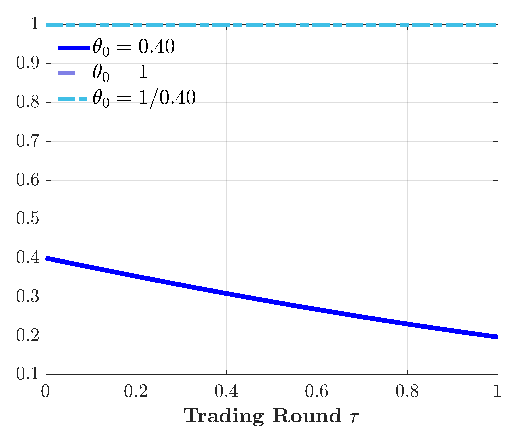
\includegraphics[width=1\linewidth]{NewCode/Figures/F_l_gammaplus_tau.eps}
\center{(a) Rate $\psi^{+}$}\endminipage\minipage{0.3\textwidth}
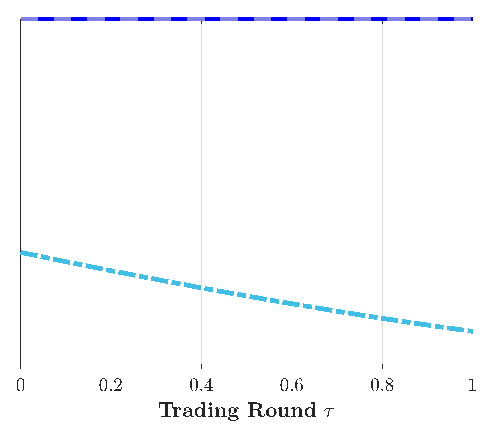
\includegraphics[width=1\linewidth]{NewCode/Figures/F_l_gammaminus_tau.eps}
\center{(b) Rates $\psi^{-}$}\endminipage\minipage{0.3\textwidth}
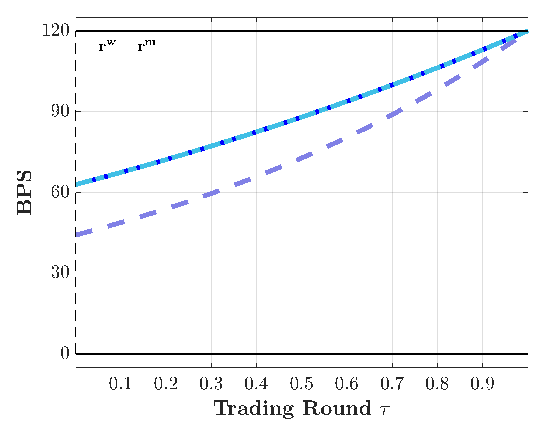
\includegraphics[width=1\linewidth]{NewCode/Figures/F_l_Surplus_tau.eps}
\center{(c) Surplus $\Sigma_{\tau}$} \endminipage
\par\end{centering}
\centering{}\minipage{0.3\textwidth}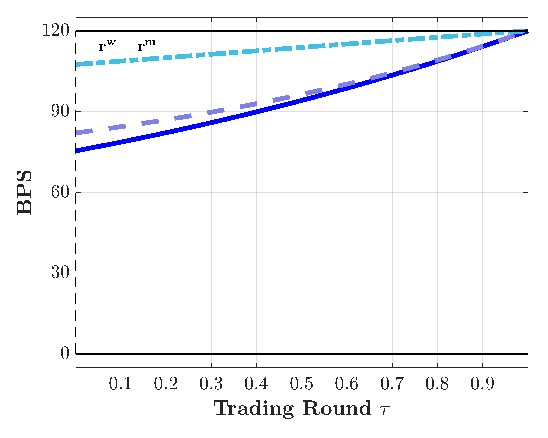
\includegraphics[width=1\linewidth]{NewCode/Figures/F_l_Chiminus_tau.eps}
\center{(d) Cost $\chi^{-}$} \endminipage\minipage{0.3\textwidth}
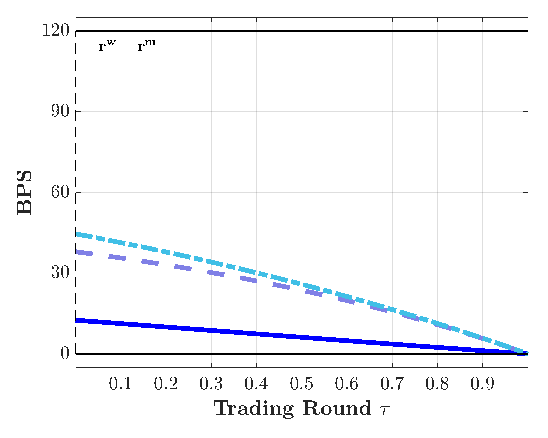
\includegraphics[width=1\linewidth]{NewCode/Figures/F_l_Chiplus_tau.eps}
\center{(e) Benefit $\chi^{+}$} \endminipage\minipage{0.3\textwidth}
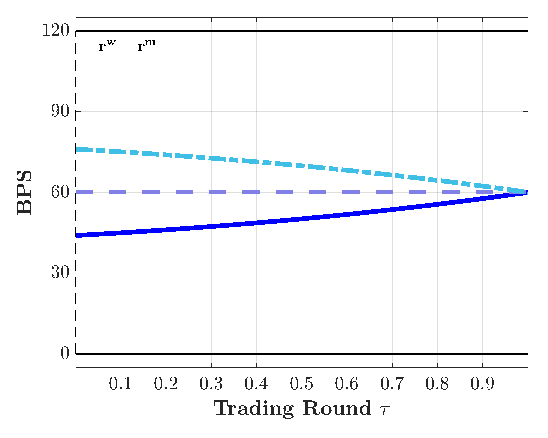
\includegraphics[width=1\linewidth]{NewCode/Figures/F_l_InterbankRate_tau.eps}
\center{(f) Rate $r^{f}_{\tau}$} \endminipage
\end{figure}
\end{frame}

\begin{frame}{Example: Cobb-Douglas $G(a, b) = \sqrt{a\cdot b}$}

%$\eta = 0.5$, $\bar{\lambda} = 1.2$, $r^w - r^m = 120$bps
\begin{figure}[t!]
\begin{centering}
\minipage{0.3\textwidth} 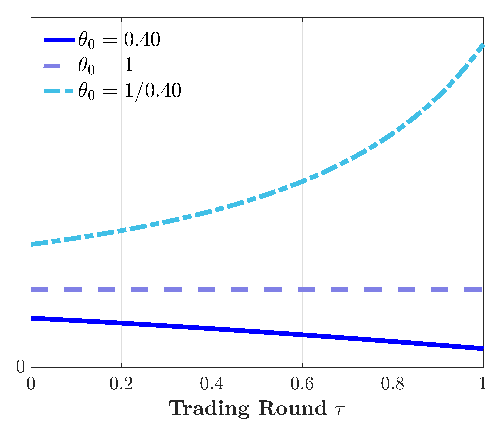
\includegraphics[width=1\linewidth]{NewCode/Figures/F_cd_gammaplus_tau.eps}
\center{(a) Rate $\psi^{+}$}\endminipage\minipage{0.3\textwidth}
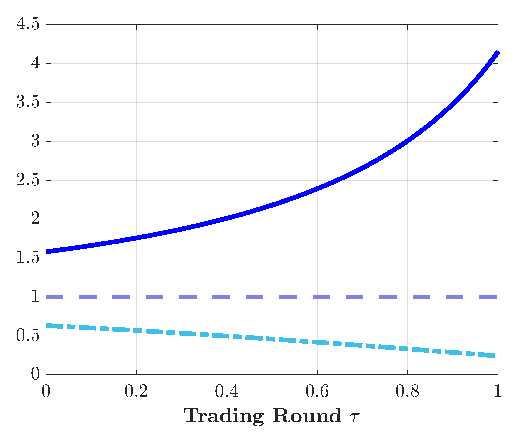
\includegraphics[width=1\linewidth]{NewCode/Figures/F_cd_gammaminus_tau.eps}
\center{(b) Rates $\psi^{-}$}\endminipage\minipage{0.3\textwidth}
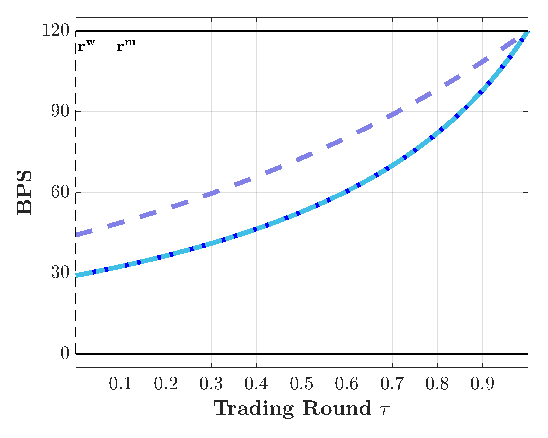
\includegraphics[width=1\linewidth]{NewCode/Figures/F_cd_Surplus_tau.eps}
\center{(c) Surplus $\Sigma_{\tau}$} \endminipage
\par\end{centering}
\centering{}\minipage{0.3\textwidth}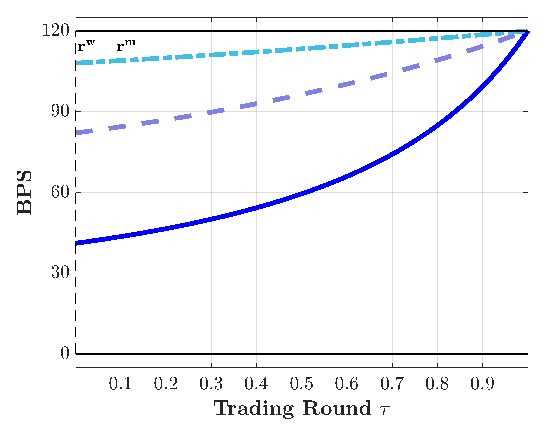
\includegraphics[width=1\linewidth]{NewCode/Figures/F_cd_Chiminus_tau.eps}
\center{(d) Cost $\chi^{-}$} \endminipage\minipage{0.3\textwidth}
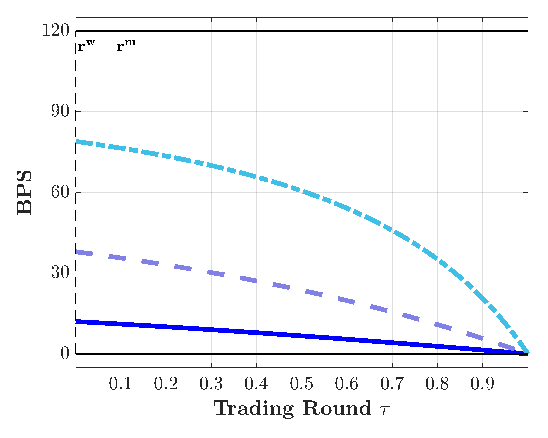
\includegraphics[width=1\linewidth]{NewCode/Figures/F_cd_Chiplus_tau.eps}
\center{(e) Benefit $\chi^{+}$} \endminipage\minipage{0.3\textwidth}
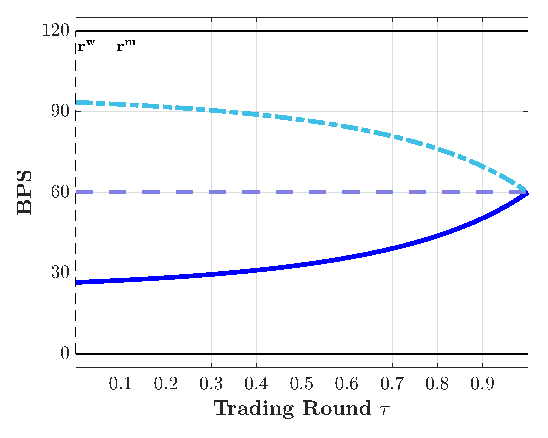
\includegraphics[width=1\linewidth]{NewCode/Figures/F_cd_InterbankRate_tau.eps}
\center{(f) Rate $r^{f}_{\tau}$} \endminipage
\end{figure}
\end{frame}

\subsection{Properties}

\begin{frame}{Four Properties}
%\begin{block}{ Core Insights}
\begin{itemize}
  \item \textbf{Balanced market}  
  balanced market ($\theta_0 = 1$), stays balanced. 
  \begin{itemize}
  \item Exogenous trading probs.
  \end{itemize}
    \medskip
  \item \textbf{Time Dilation}  
  Dynamics from any point in session
\begin{itemize}
  \item  Reset to full session, scale matching efficiency $\bar{\lambda}$ remaining time
  \end{itemize}
 
 \medskip
  \item \textbf{Symmetry}  
  Swapping deficit and surplus sides ($\theta \leftrightarrow \theta^{-1}$, $\eta \leftrightarrow 1 - \eta$)
  \begin{itemize}
    \item  mirrors yields around $r^w - r^m$
  \end{itemize}
  
 \medskip
  \item \textbf{Bargaining Power} Borrower power ($\eta \uparrow$) lowers rates and yield coefficients
  \begin{itemize}
    \item  full borrower power $\Rightarrow \bar{r}^f = r^m$, viceversa
  \end{itemize}
  
\end{itemize}
% \end{block}
\end{frame}

\begin{comment}
\begin{frame}{Properties of Tightness in Continuous Time}
\begin{block}{Proposition}
\begin{itemize}
  \item $\theta_0 = 1 \Rightarrow \theta_\tau = 1$
  \item $\theta_0 > 1$ increases, $\theta_0 < 1$ decreases
  \item Higher $\gamma(\theta)$ speeds convergence
\end{itemize}
\end{block}
\end{frame}

\begin{frame}{Time Dilation Property}
\begin{block}{Proposition (Time Dilation)}
Fix $\tau, \tau' \in [0,1]$ with $\tau' > \tau$. Then:
\[
\theta\left(\tau', \theta_0, \bar{\lambda}\right) = \theta\left(\frac{\tau' - \tau}{1 - \tau}, \theta(\tau, \theta_0, \bar{\lambda}), \bar{\lambda}(1 - \tau)\right)
\]
Same holds for: $\{\psi^\pm, r^f, \Sigma, \chi^\pm\}$.
\end{block}
\begin{itemize}
  \item Recursive computation of tightness
  \item Properties at one point generalize to all
  \item Normalization to $[0,1]$ is without loss
\end{itemize}
\end{frame}

\begin{frame}{Symmetry Property}
\begin{block}{Proposition (Symmetry)}
For all $\theta, \eta, \bar{\lambda}$:
\begin{align*}
\Sigma(\tau, \theta, \eta) &= \Sigma(\tau, \theta^{-1}, 1 - \eta) \\
  r^f(\tau, \theta, \eta) &= (r^w - r^m) - r^f(\tau, \theta^{-1}, 1 - \eta) \\
  \chi^-(\tau, \theta, \eta) &= (r^w - r^m) - \chi^+(\tau, \theta^{-1}, 1 - \eta) \\
  \chi^+(\tau, \theta, \eta) &= (r^w - r^m) - \chi^-(\tau, \theta^{-1}, 1 - \eta)
\end{align*}
\end{block}
\begin{itemize}
  \item Results for $\theta > 1$ mirror $\theta < 1$
  \item Rate and yield functions centered around $r^w - r^m$
\end{itemize}
\end{frame}
\end{comment}

\begin{frame}{Efficiency Limits}
The OTC market equilibrium satisfies:
\begin{itemize}
  \item \textbf{Walrasian Limit ($\bar{\lambda} \to \infty$)}
  \begin{itemize}
    \item $\theta > 1$: $\Psi^+ = 1$, $\Psi^- = 1/\theta$, $\chi^+ = \chi^- = r^w - r^m$
    \item $\theta < 1$: $\Psi^+ = \theta$, $\Psi^- = 1$, $\chi^+ = \chi^- = 0$
    \item $\theta = 1$: $\Psi^+ = \Psi^- = 1$, $\chi^+ = \chi^- = (1 - \eta)(r^w - r^m)$
  \end{itemize}
  \medskip
  \item \textbf{Static Limit ($\bar{\lambda} \to 0$)}
  \begin{itemize}
    \item $\Psi^+ = \Psi^- = 0$, $\chi^+ = 0$, $\chi^- = r^w - r^m$
    \item $\overline{r}^f = r^m + (1 - \eta)(r^w - r^m)$
  \end{itemize}
\end{itemize}
%\end{block}
\medskip
\begin{itemize}
  \item High efficiency leads to Walrasian outcomes
  \item Low efficiency: bargaining as in one round
\end{itemize}
\end{frame}

\begin{comment}
\begin{block}{Illustration}
\textbf{Panel (a): Symmetry.} Yield coefficients $\chi^+$, $\chi^-$ for varying $\log(\theta_0)$, $
\quad\eta \in \{0.25, 0.5, 0.75\}$. 180$^\circ$ rotation yields same curves under $\eta \leftrightarrow 1 - \eta$.

\textbf{Panel (b): Walrasian Limit.} As $\bar{\lambda} \to \infty$, $r^f_\tau \to r^m$, matching frictions vanish.
\end{block}
\end{comment}

\begin{frame}{Symmetry and Walrasian Limit}

\begin{figure}
\begin{minipage}[b]{.4\linewidth}
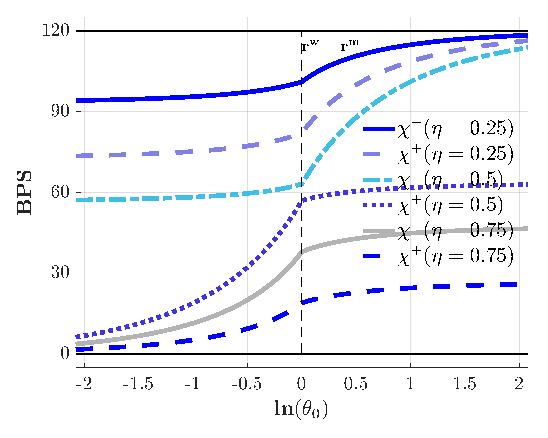
\includegraphics[width=1.1\linewidth]{NewCode/Figures/F_l_symmetry_theta.eps}
\center{(a) Symmetry Property}
\end{minipage}
\hspace{1cm}
   \begin{minipage}[b]{.4\linewidth}
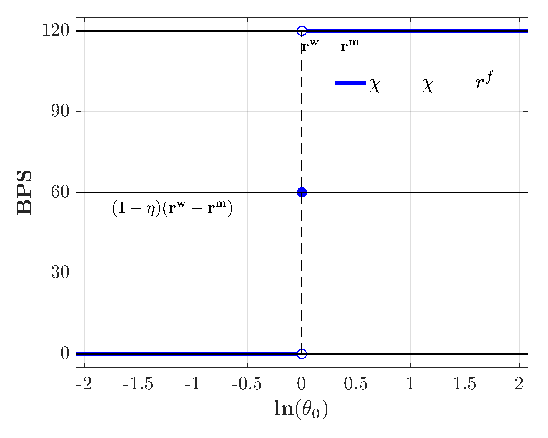
\includegraphics[width=1.1\linewidth]{NewCode/Figures/F_Walrasian_prices_theta.eps}
\center{(b) Walrasian Limit}
\end{minipage}
\end{figure}
\end{frame}

\begin{frame}{Market Tightness}
\begin{itemize}
  \item $\chi^+, \chi^-, \overline{r}^f$ increasing in tightness $\theta$
  \item What about extrema?
  \medskip
\end{itemize}  
\begin{block}{Proposition (Extrema of Market Tightness)}
  \begin{itemize}
  \item $\theta \to 0$: $\chi^+ \to 0$, $\chi^- \to (r^w - r^m)e^{-\bar{\lambda}\bar{\gamma}\eta}$
  \item $\theta \to \infty$: $\chi^- \to r^w - r^m$, $\chi^+ \to (r^w - r^m)(1 - e^{-(1 - \eta)\bar{\lambda}\bar{\gamma}})$
\end{itemize}
\end{block}
\medskip
\begin{itemize}
  \item \textbf{Key:} boundedness \alert{$\bar{\gamma}$} = $\lim_{\theta \to 0} \gamma(\theta^{-1})$
  \item \textbf{$\bar{\gamma}$ finite:} yields/rates stay positive even as $\theta \to 0$
  
  
\end{itemize}
\end{frame}

\begin{frame}{The CES Matching Class}

\begin{itemize}
  \item CES: $G(a,b)=(a^p+b^p)^{1/p}$, $p\leq 0$
   \medskip   
  \item Within CES: Cobb-Douglas ($p=0$) is knife-edge 
  \begin{itemize}
  \item Only matching function $\theta_\tau$ can reach 0 in finite time
  \item We care because Cobb-Douglas allows zero convenience yields
  \end{itemize}
  
\end{itemize}
\end{frame}

\begin{frame}{The CES Matching Class}
\begin{figure}[h!]
    \begin{minipage}[b]{.35\linewidth} 
        \center{(a)  Growth rate of $\theta_{\tau}$}
        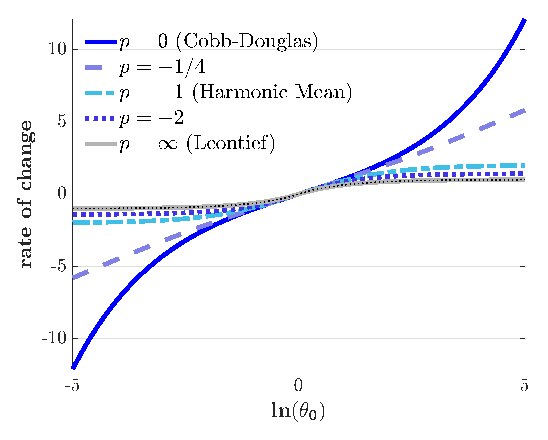
\includegraphics[width=1\linewidth]{NewCode/Figures/F_growthrate.eps}
    \end{minipage}
   \hspace{1cm}
    \begin{minipage}[b]{.35\linewidth}
    \center{(b) Evolution of $\theta_{\tau}$}
    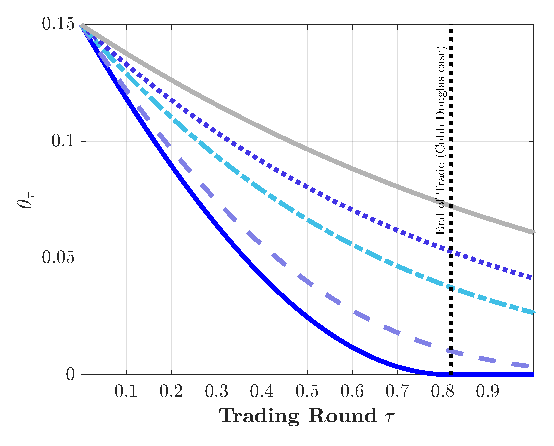
\includegraphics[width=1\linewidth]{NewCode/Figures/F_trajectories.eps}
    \end{minipage}

\begin{minipage}[b]{.35\linewidth}
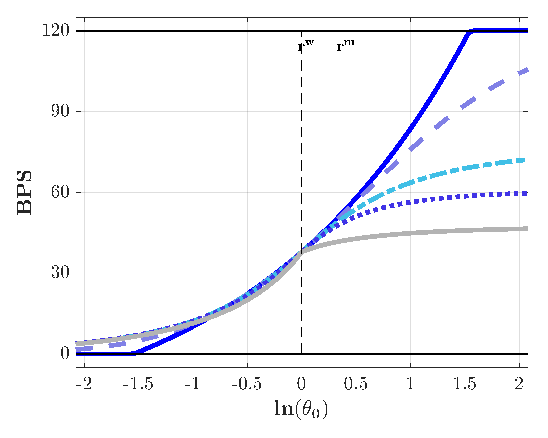
\includegraphics[width=1\linewidth]{NewCode/Figures/F_chip_comp.eps}
\center{(c) $\chi^{+}$}
\end{minipage}
 \hspace{1cm}
\begin{minipage}[b]{.35\linewidth}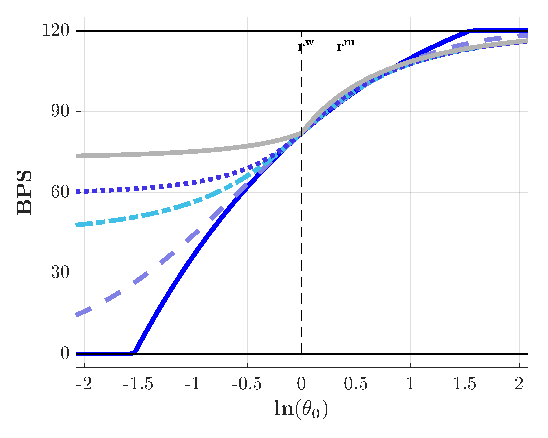
\includegraphics[width=1\linewidth]{NewCode/Figures/F_chim_comp.eps}
\center{(d) $\chi^{-}$}
\end{minipage}
\caption{\label{fig:F_comparison}\textbf{Comparison Across CES matching functions.
}}

\parbox[b]{16cm}{\small \emph{Note:} $\theta=\theta_{0}$ is the initial market tightness. The example
is calibrated with $\eta=0.5$, $\bar{\lambda}=1.2$, $r^{w}-r^{m}=120$bps
in all cases.}
\end{figure}

\end{frame}

\subsection{Fully Analytic Cases}

\begin{frame}{Tightness Formula: Cobb-Douglas vs. Leontief}
{\tiny
\begin{block}{Market Tightness $\theta(\tau)$}
\begin{tabular}{|l|c|c|}
\hline
\textbf{Feature} & \textbf{Cobb-Douglas ($p=0$)} & \textbf{Leontief ($p=-\infty$)} \\
\hline
$\theta(\tau)$ & $\left(\frac{(1+\sqrt{\theta_0})e^{-\bar{\lambda} \tau} - (1-\sqrt{\theta_0})}{(1+\sqrt{\theta_0})e^{-\bar{\lambda} \tau} + (1-\sqrt{\theta_0})}\right)^2$ & $\begin{cases} 1 + (\theta_0 - 1)e^{\bar{\lambda} \tau}, & \theta_0 > 1 \\ \theta_0 / (\theta_0 + (1 - \theta_0)e^{\bar{\lambda} \tau}), & \theta_0 < 1 \end{cases}$ \\
\hline
Stop $T$ & $\min\left\{ \frac{1}{\bar{\lambda}} \log\left(\left|\frac{1 + \sqrt{\theta_0}}{1 - \sqrt{\theta_0}}\right|\right),\,1\right\}$ & $\infty$ \\
\hline
$\Psi^+$ & $1-e^{-\bar{\lambda}T}\left(\frac{(1+\sqrt{\theta_0})+(1-\sqrt{\theta_0})e^{\bar{\lambda}T}}{(1+\sqrt{\theta_0})+(1-\sqrt{\theta_0})}\right)^2$ & $\begin{cases} 1 - e^{-\bar{\lambda}}, & \theta_0 \geq 1 \\ \theta_0(1 - e^{-\bar{\lambda}}), & \theta_0 < 1 \end{cases}$ \\
\hline
$\Psi^-$ & $1-e^{-\bar{\lambda}T}\left(\frac{(1+\sqrt{\theta_0})-(1-\sqrt{\theta_0})e^{\bar{\lambda}T}}{(1+\sqrt{\theta_0})-(1-\sqrt{\theta_0})}\right)^2$ & $\begin{cases} (1 - e^{-\bar{\lambda}})\theta_0^{-1}, & \theta_0 > 1 \\ 1 - e^{-\bar{\lambda}}, & \theta_0 \leq 1 \end{cases}$ \\
\hline
\end{tabular}
\end{block}
}
\end{frame}

\begin{frame}{Closed-Form: Yields and OTC Rate}
Set $\bar{\theta}=\theta_1$ and $\theta=\theta_0$
\begin{block}{Yield Coefficients and OTC Rate}
For both Cobb-Douglas and Leontief:
\[
\chi^+ = (r^w - r^m)\left(\frac{\bar{\theta} - \bar{\theta}^\eta \theta^{1 - \eta}}{\bar{\theta} - 1}\right),\quad
\chi^- = (r^w - r^m)\left(\frac{\bar{\theta} - \bar{\theta}^\eta \theta^{-\eta}}{\bar{\theta} - 1}\right)
\]
\[
\overline{r}^f = \phi(\theta) r^m + (1 - \phi(\theta)) r^w, \quad \phi(\theta) = \frac{(\bar{\theta}/\theta)^\eta - \theta}{\bar{\theta}/\theta - 1}
\]
\end{block}
\begin{itemize}
  \item $\phi(\theta)$ acts as \textbf{endogenous bargaining index}
  \item Valid in closed-form only for $p = 0$ and $p = -\infty$ 
  \begin{itemize}
  \item but not for all p
  \end{itemize}
\end{itemize}
\end{frame}

\begin{frame}{Cobb-Douglas vs. Leontief}
%\begin{block}{Figure: $\chi^+, \chi^-, \overline{r}^f$ across $\log(\theta_0)$}
%Comparative statics across the two polar CES cases. Rates and yield coefficients evolve differently as a function of initial market tightness.
%\end{block}
\begin{minipage}{0.48\textwidth}
  \centering
  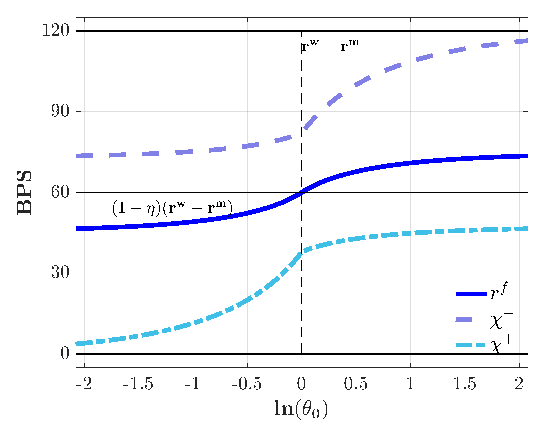
\includegraphics[width=0.95\textwidth]{NewCode/Figures/F_l_prices_theta.eps} \\
  (a) Frictional Case (Leontief)
\end{minipage}
%\hspace{1cm}
\begin{minipage}{0.48\textwidth}
  \centering
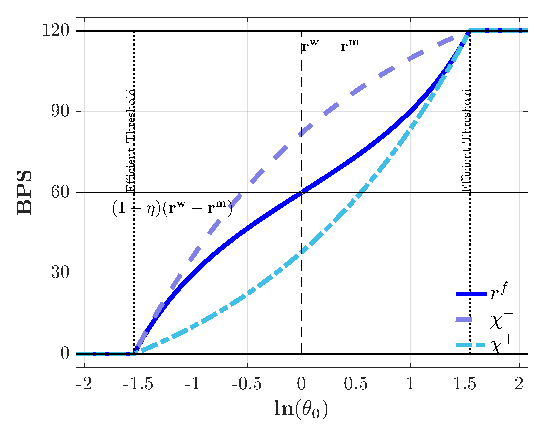
\includegraphics[width=0.95\textwidth]{NewCode/Figures/F_cd_prices_theta.eps} \\
  (b) Frictional Case (Cobb-Douglas)
\end{minipage}
\medskip
\begin{itemize}
\item T takes care of making $\theta=0$ of T<1
\end{itemize}
\end{frame}

% \setbeamertemplate{blocks}[rounded][shadow=false]

\section{Applications}

\subsection{Portfolio Choice/Asset Pricing}
% \setbeamertemplate{blocks}[rounded][shadow=false]


\begin{frame}{Portfolio Problem with Settlement Risk}
\begin{block}{Investor Preferences and Problem}
Investor solves:
\[
\max_{\{c, \tilde{a}^{i}_{t+1}, \tilde{m}_{t+1}\}} \mathbb{E}_0 \sum_{t=0}^\infty \beta^t \frac{c_t^{1-\gamma}-1}{1-\gamma}
\]
subject to budget and return constraints.
\begin{itemize}
  \item Cash return $R^m$ and asset returns $R^i$ are exogenous.
  \item Only OTC rate $\bar{R}^f$ and $\chi(s;\theta)$ endogenous
  \item Portfolio separation holds
\end{itemize}
\end{block}
\end{frame}

\begin{frame}{Return on Portfolio and Risk}
\begin{block}{Portfolio Objective}
Investor chooses weights to maximize equity return:
\[
\max_{m, a^i} \left(\mathbb{E}\left[R^e\right]^{1-\gamma}\right)^{\frac{1}{1-\gamma}}
\]
where:
\[
R^e = \sum_i R^i a^i + R^m m + \chi\left(s(a^i, m, \omega); \theta\right)
\]
\end{block}
\medskip
\begin{itemize}
  \item $\chi(s)$ is kinked: costly to be in deficit, modest benefit in surplus.
  \item $s$ depends on portfolio weights and liquidity shocks.
\end{itemize}
\end{frame}

\begin{frame}{Convenience Yields and Portfolio Premia}
\begin{block}{Decomposition of Excess Returns}
At optimality:
\begin{align*}
\mathbb{E}[R^i] - R^m &= \underbrace{-\mathbb{E}[\chi_s(\partial_m s - \partial_{a^i}s)]}_{\text{first-order liquidity yield}} \\
&\quad - \underbrace{\frac{\text{Cov}[R_e^{-\gamma}, R^i + \chi_s(\partial_m s - \partial_{a^i}s)]}{\mathbb{E}[R_e^{-\gamma}]}}_{\text{total risk premium}}
\end{align*}
\end{block}
\begin{itemize}
  \item $\chi_s$ is the marginal convenience yield ($\chi^+$ or $\chi^-$).
  \item \textbf{Lesson:} premia reflect both mean liquidity effects and covariance with risk.
  \begin{itemize}
  \item Risk and liquidity, not decoupled!
  \item FX literature: assumes they are
  \end{itemize}
\end{itemize}
\end{frame}

\begin{frame}{Lessons for Portfolio Theory}
%\begin{itemize}
  Convenience yields:
  \begin{itemize}
  \item force toward determinate portfolios even under risk neutrality
  \end{itemize}
  \medskip
     Risk premia vs. convenience yield decompositions:
    \begin{itemize}
    \item not decoupled
    \end{itemize}
    \medskip
   Applications: Pricing anomalies
  \begin{itemize}
    \item short-term rate puzzle (Lenel-Piazzesi-Schneider)
    \item corporate-rate puzzle (Liao)
    \item CIP deviations (Krishnarmurthy-Jian-Lustig)
    \item deposit-rate heterogeneity (Dreschler-Savov-Schnabl)
 \end{itemize}
%\end{itemize}
\end{frame}

\subsection{Identification}
\begin{frame}{What Are We Trying to Identify?}
\begin{block}{Three Key Parameters}
\begin{itemize}
  \item Market tightness $\theta$: imbalance between buyers and sellers
  \item Matching efficiency $\bar{\lambda}$: how quickly matches form
  \item Bargaining power $\eta$: who keeps the surplus
\end{itemize}
\end{block}
\vspace{0.2cm}
\begin{itemize}
  \item Why identify them?
  \begin{itemize}
    \item Decompose sources of convenience yields
    \item Run policy or institutional counterfactuals
    \item Map observed premia to underlying frictions
  \end{itemize}
\end{itemize}
\end{frame}

\begin{frame}{Non-Monotonicity: Identification Challenge}
\begin{figure}[b!]

   \begin{minipage}[b]{.49\linewidth} 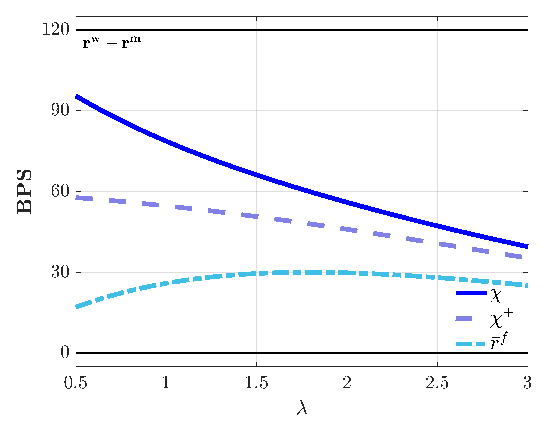
\includegraphics[width=1\linewidth]{NewCode/Figures/F_l_prices_lambda.eps}\center{(a) Leontief Matching}\end{minipage}\hfill{}  
   \begin{minipage}[b]{.49\linewidth}
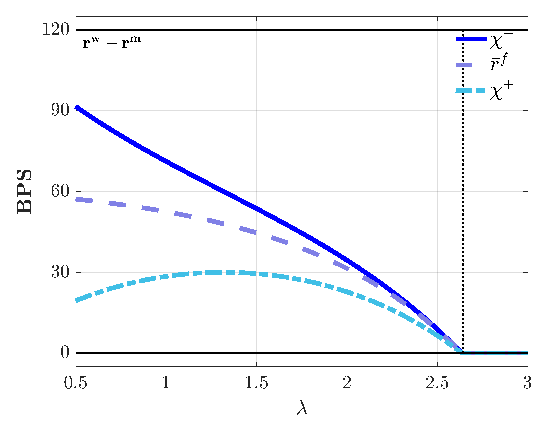
\includegraphics[width=1\linewidth]{NewCode/Figures/F_cd_prices_lambda.eps}
\center{(b) Cobb-Dogulas Matching}\end{minipage}
\medskip
\begin{itemize}
\item Non monotonic yields in efficiency
\end{itemize}
\end{figure}
\end{frame}

\begin{frame}{Identification Strategy: Moments and Mapping}
\begin{block}{Observable Moments}
\begin{itemize}
  \item $\bar{r}^f$ and $\chi^\pm$ \(\Rightarrow\) pin down $\theta$ (monotonicity)
  \item Portfolios and implied $\theta$ \(\Rightarrow\) shock distribution $\Phi$
  \item Intraday dispersion $Q$ \(\Rightarrow\) moment identify $\bar{\lambda}$ or G
  \item Relative volume $I(\theta)\equiv\frac{\Psi^{-}}{1-\Psi^{-}}$ \(\Rightarrow\) clean moment for $\bar{\lambda}$
  \item Use $\chi^+/\chi^-$ near $\theta=1$ \(\Rightarrow\) infer $\eta$
\end{itemize}
\end{block}

\end{frame}

\begin{frame}{Identification Strategy: Moments and Mapping}

\begin{block}{Observable Moments}
\begin{itemize}
  \item $\bar{r}^f$ and $\chi^\pm$ \(\Rightarrow\) pin down $\theta$ (monotonicity)
  \item Portfolios and implied $\theta$ \(\Rightarrow\) shock distribution $\Phi$
  \item Intraday dispersion $Q$ \(\Rightarrow\) moment identify $\bar{\lambda}$ or G
  \item Relative volume $I(\theta)\equiv\frac{\Psi^{-}}{1-\Psi^{-}}$ \(\Rightarrow\) clean moment for $\bar{\lambda}$
  \item Use $\chi^+/\chi^-$ near $\theta=1$ \(\Rightarrow\) infer $\eta$
\end{itemize}
\end{block}

\end{frame}

\begin{frame}{Payoff}
\begin{itemize}
  \item Estimate of $\frac{R^f-R^m}{R^w-R^m}$ as function of $\theta(M/D)$ for Euro Area
  \item Used in Bigio-Linzert-Mendo-Schumacher-Thaler:
\end{itemize}
\begin{figure}[b!]
  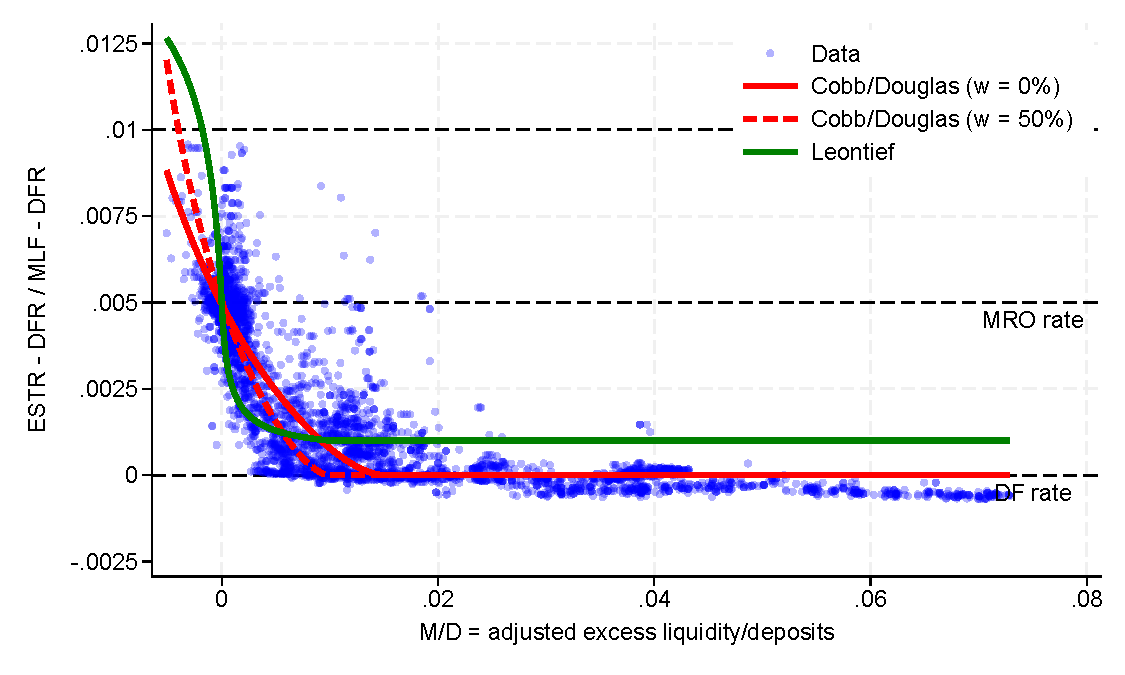
\includegraphics[width=0.6\linewidth]{NewCode/Figures/Fitted_RfRm_Europe.pdf}\center{Fit to Euro Area}
  \end{figure}
\end{frame}

\subsection{Efficiency}

\begin{frame}{Efficiency}

\begin{itemize}
  \item Portfolio choice may be constrained inefficient
  \item Depends on who earns penalties
  \item Here, assume it's waste
\end{itemize}

\end{frame}

\begin{frame}{Banking Example: Withdrawal Risk}
\begin{block}{Portfolio Structure in Bianchi-Bigio '22}
\begin{itemize}
  \item Assets: cash $m$, illiquid bond $b$.
  \item Liability: deposit $d$ subject to withdrawal shock $\omega$.
  \item Settlement position:
  \[
  s(b, d, m) = m + \left(\frac{R^d}{R^m}\omega - \rho(1+\omega)\right)d
  \]
  \item Budget: $b + m = 1 + d$.
\end{itemize}
\end{block}
\end{frame}

\begin{comment}
\begin{frame}{Withdrawal Risk Optimization}
\begin{block}{Investor Problem}
\[
\max_{m \geq 0, d \geq 0} \left\{ \mathbb{E}_{\omega}\left[R^b + R^b(d - m) + R^m m - R^d d + \chi(s(d,m);\theta)\right]^{1 - \gamma} \right\}^{1/(1 - \gamma)}
\]
\end{block}
\begin{itemize}
  \item Settlement risk reflected in $\chi(s(d,m);\theta)$.
  \item Risk-adjusted premia emerge from the structure of $s$ and $\chi$.
\end{itemize}
\end{frame}
\end{comment}

\begin{frame}{Liquidity Premium on Bonds}
\begin{block}{Illiquid Asset vs. Cash}
\[
R^b - R^m = \chi^+ + (\chi^- - \chi^+)\tilde{\Phi}(\omega^*)
\]
where:
\[
\tilde{\Phi}(\omega^*) = \Phi(\omega^*) \cdot \frac{\mathbb{E}[R^e(\omega)^{-\gamma} | \omega < \omega^*]}{\mathbb{E}[R^e(\omega)^{-\gamma}]},\quad \omega^* = \frac{\rho - m/d}{R^d/R^m - \rho}
\]
\end{block}
\begin{itemize}
  \item $\Phi(\omega^*)$: probability of cash deficit.
  \item $\tilde{\Phi}$: risk-adjusted deficit probability.
\end{itemize}
\end{frame}

\begin{comment}
\begin{frame}{Liquidity Premium on Deposits}
\begin{block}{Illiquid Asset vs. Deposits}
\[
R^b - R^d = \chi^+ + (\chi^- - \chi^+)\tilde{\Phi}(\omega^*)\left(\left(\frac{R^d}{R^m} - \rho\right)\mathbb{E}[\omega R^e(\omega)^{-\gamma} | \omega < \omega^*] - \rho\right)
\]
\end{block}
\begin{itemize}
  \item Captures the tail risk of deposit withdrawals.
  \item Liquidity premium increases with withdrawal exposure.
\end{itemize}
\end{frame}
\end{comment}

\begin{frame}{Efficiency of Portfolio Management}
\begin{itemize}
\item Investors: not internalize effect on market tightness $\theta$
\medskip
\item Externality: cash  improves reduces external borrowing + but has opportunity cost
\item Haider-Ismail and Zuniga
\begin{itemize}
\item flipside, study loan-deposit wedge with rebate
\end{itemize}
\end{itemize}
\end{frame}

\begin{frame}{Planner Problem}
\begin{block}{Planner Optimality Condition}
$R^b - R^m = \chi^+ + (\chi^- - \chi^+) \tilde{\Phi}(\omega^*) + H$
\begin{itemize}
\item $H$: pecuniary externality from $m$'s effect on $\theta$ and $\chi$.
\item Planner internalizes how $m$ affects matching and yields.
\end{itemize}
\end{block}
\end{frame}

\begin{frame}{Direction of the Externality}
\begin{itemize}
\item Risk-neutrality ($\gamma \to 0$), planner values cash more iff
\[
\text{ } \alert{\frac{\partial \chi^+}{\partial \theta} S^+ > \frac{\partial \chi^-}{\partial \theta} S^-}
\]

\end{itemize}
\end{frame}

\begin{frame}{Cases: Leontief vs. Cobb-Douglas}
\begin{itemize}
\item Cobb-Douglas: 
\begin{itemize}
\item near balanced market ($\theta=1$),  no inefficiency.
\item risk-aversion: force toward more liquidity $m$ $\Rightarrow$ precautionary motive
\end{itemize}
\medskip
\item Leontief: 
\begin{itemize}
\item matching probabilities of short-side fixed
\item no inefficiency if planner \& market allocation feature aggregate surplus
\end{itemize}
\medskip
\item Inefficiencies: matching-function specific
\end{itemize}
\end{frame}

\begin{comment}
\item Static OTC markets: Inefficiency depends on surplus vs. deficit side.
\item With excess deficits: planner values $m$ more than private investors.
\item With excess surplus: planner values $m$ less.
\end{comment}

\begin{frame}{Policy Implications}
\begin{itemize}
\item Inefficiency: liquidity regulation
\item Planner: more cash to reduce exposure to costly borrowing (e.g., FX reserve management, Central Bank balance sheet)
\end{itemize}
\end{frame}

\section{Conclusion}

\begin{frame}{Limitations and Extensions}
\begin{itemize}
  \item Results rely on simplifying assumptions
  \begin{itemize}
  \item large number of traders, no network, no effort
  \end{itemize}
  
  \medskip
  \item Portfolio: one layer. Reality: multi-layered.
  \medskip
  \item \alert{\textbf{Still, useful to know simplest outcomes}}
\end{itemize}
\end{frame}

\begin{frame}{Thank You!}
\begin{center}
  Questions, comments?
\end{center}
\end{frame}

\end{document}

